\subsection*{Kvalitetsscenarier}
Her er de forskellige kvalitetsscenarier vi forventer kan have relevans for systemet. \\

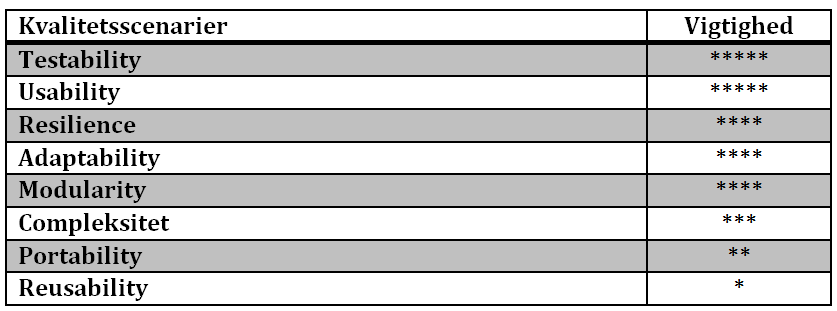
\includegraphics[scale=0.60]{includes/billeder/kvalitetsscenarietabel.png}

\textsc{Termer:} \\ \\

Testability/testbart: \\
Funktionaliteten for skal v�re testbar for at kunne sikre usability. \\

Usability/brugbarhed: \\
Appen skal v�re nem at bruge for at den adskiller sig fra andre apps indenfor markedet. \\

Resilience/modstandsdygtigt: \\
Systemet skal kunne komme op at k�re hurtigt igen efter problemer. \\

Adaptability/tilpasseligt: \\
Systemet skal nemt kunne tilpasses i forhold til udvikling af nyt system eller krav�ndringer. \\

Modularity/modul�rt:\\ 
Det er vigtigt at systemet er modul�rt for at sikre adaptability og scalability.\\

Complexity/komplekst: \\
For at appen kan blive tilpas nem at bruge og adskille sig fra andre lignende apps er kompleksitet er n�dvendighed is�r i forhold til FoodMappet samt eventuelle algoritmer til at give brugeren relevante forslag til ingredienser og opskrifter. \\

Portability/overf�rlighed:\\ 
P� l�ngere sigt er det vigtigt at appen kan portes til andre platforme, men i f�rste omgang vil det v�re en fordel at fokusere p� en enkelt platform for at skabe en vis interesse for appen f�rst. S� kan man begynde at bruge resurser p� at porte den n�r den har vist sig at have potentiale. \\

Reusability/genbrugelighed: \\
Det er p� l�ngere sigt vigtigt at appen kan genbruges til videre udvikling fx som: diabetiker eller fitness app. \\
Samt at det ogs� vil v�re en fordel at kunne genbruge databasen til p� platforme. \\

Reliability/p�lidelighed: \\
Hvis vi havde valgt at fokusere p� en diabetiker version af appen ville det v�re meget vigtigt at brugeren kan stole p� informationen. \\

Robustness/robust: \\
Det er ikke s� vildt vigtigt at appen ikke crasher idet at den blot kan startes igen.
Dog er det vigtigt at server databaserne kan h�ndtere et vist antal foresp�rgsler n�r der opdateres med nye opskrifter. \\


%Vigtighed af kvalitetsscenarier: \\
%- Resilience: **** \\
%- Testability: ***** \\
%- Adaptability: **** \\
%- Modularity: **** \\
%- Compleksitet: *** \\
%- Portability: ** \\
%- Usability: ***** \\
%- Reusability: *

\newpage

\subsection*{Kravscenerier}
Vi har lavet kravscenerier til de 2 vigtigste stories: "Bruger vil gerne have ingrediens forslag" og "Bruger vil gerne have liste med opskrifter". \\  

\textbf{Bruger vil gerne have ingrediens forslag} \\
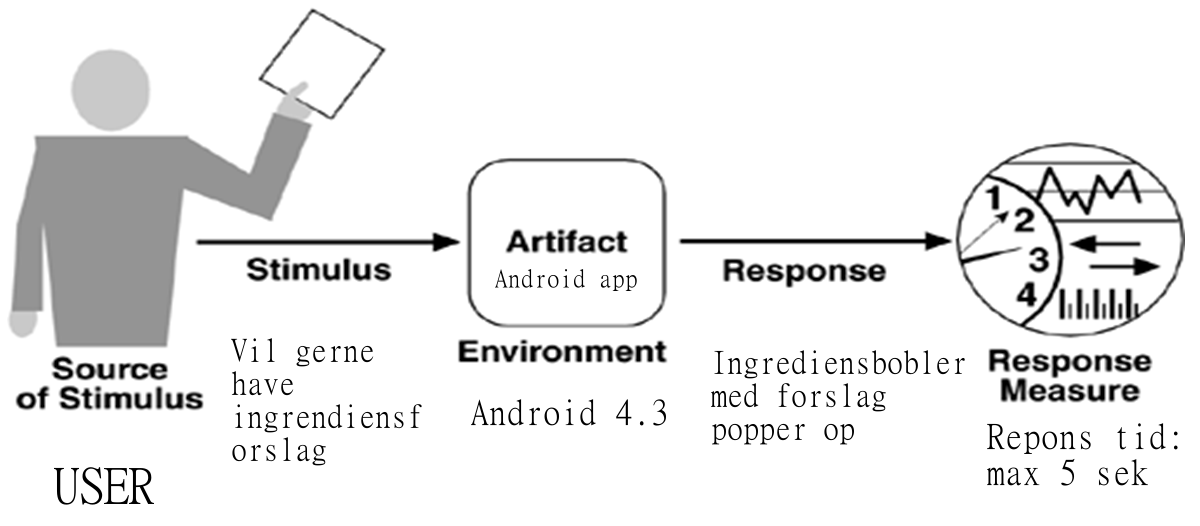
\includegraphics[scale=0.30]{includes/billeder/kravsscenerie_foodwheel.png} \\
I dette scenarie vil brugeren gerne have forslag til ingredienser. Han interagerer s� med genstanden som er en android app i milj�et Android 4.3 og f�r som respons vist grafiske bobler der indeholder forslag til ingredienser indenfor maks 5 sekunder. Den korte responstid er vigtig for at brugeren f�r en god oplevelser og ikke bliver ut�lmodig.

\textbf{Bruger vil gerne have liste med opskrifter} \\
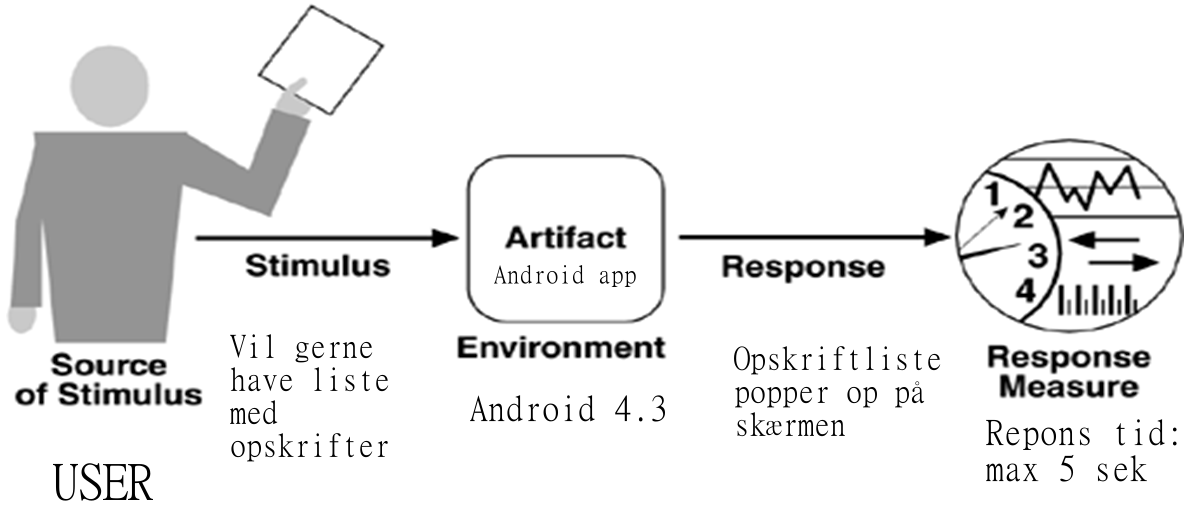
\includegraphics[scale=0.30]{includes/billeder/kravsscenerie_opskriftliste.png} \\
I dette scenarie vil brugeren gerne have en liste med forslag til opskrifter. Han interagerer s� med genstanden som er en android app i milj�et Android 4.3 og f�r som respons vist en liste af opskrifter indenfor maks 5 sekunder. Den korte responstid er vigtig for at brugeren f�r en god oplevelser og ikke bliver ut�lmodig.